% Expt Fig 1 (sister panels) + optimal-stopping companion.
% Source figures:
%   experiments/figures/10_sister_panels/expt_fig1_sister_panels.pdf
%   experiments/figures/10_sister_panels/expt_optimal_stopping.pdf
% Source table:
%   experiments/figures/10_sister_panels/stopping_exponents_table.tex
% Producer: experiments/analysis/expt_fig1_sister_panels.py
% Fits CSV: experiments/figures/10_sister_panels/expt_fig1_sister_panels_fits.csv
% Per-cell table: experiments/figures/10_sister_panels/optimal_stopping_table.csv
%
% In the ICLR manuscript these are Figure 1 (fig:datasize_sweep),
% Figure 7 (fig:optimal_stopping) and Table 1 (tab:stopping_exponents).

\begin{figure}[t]
  \centering
  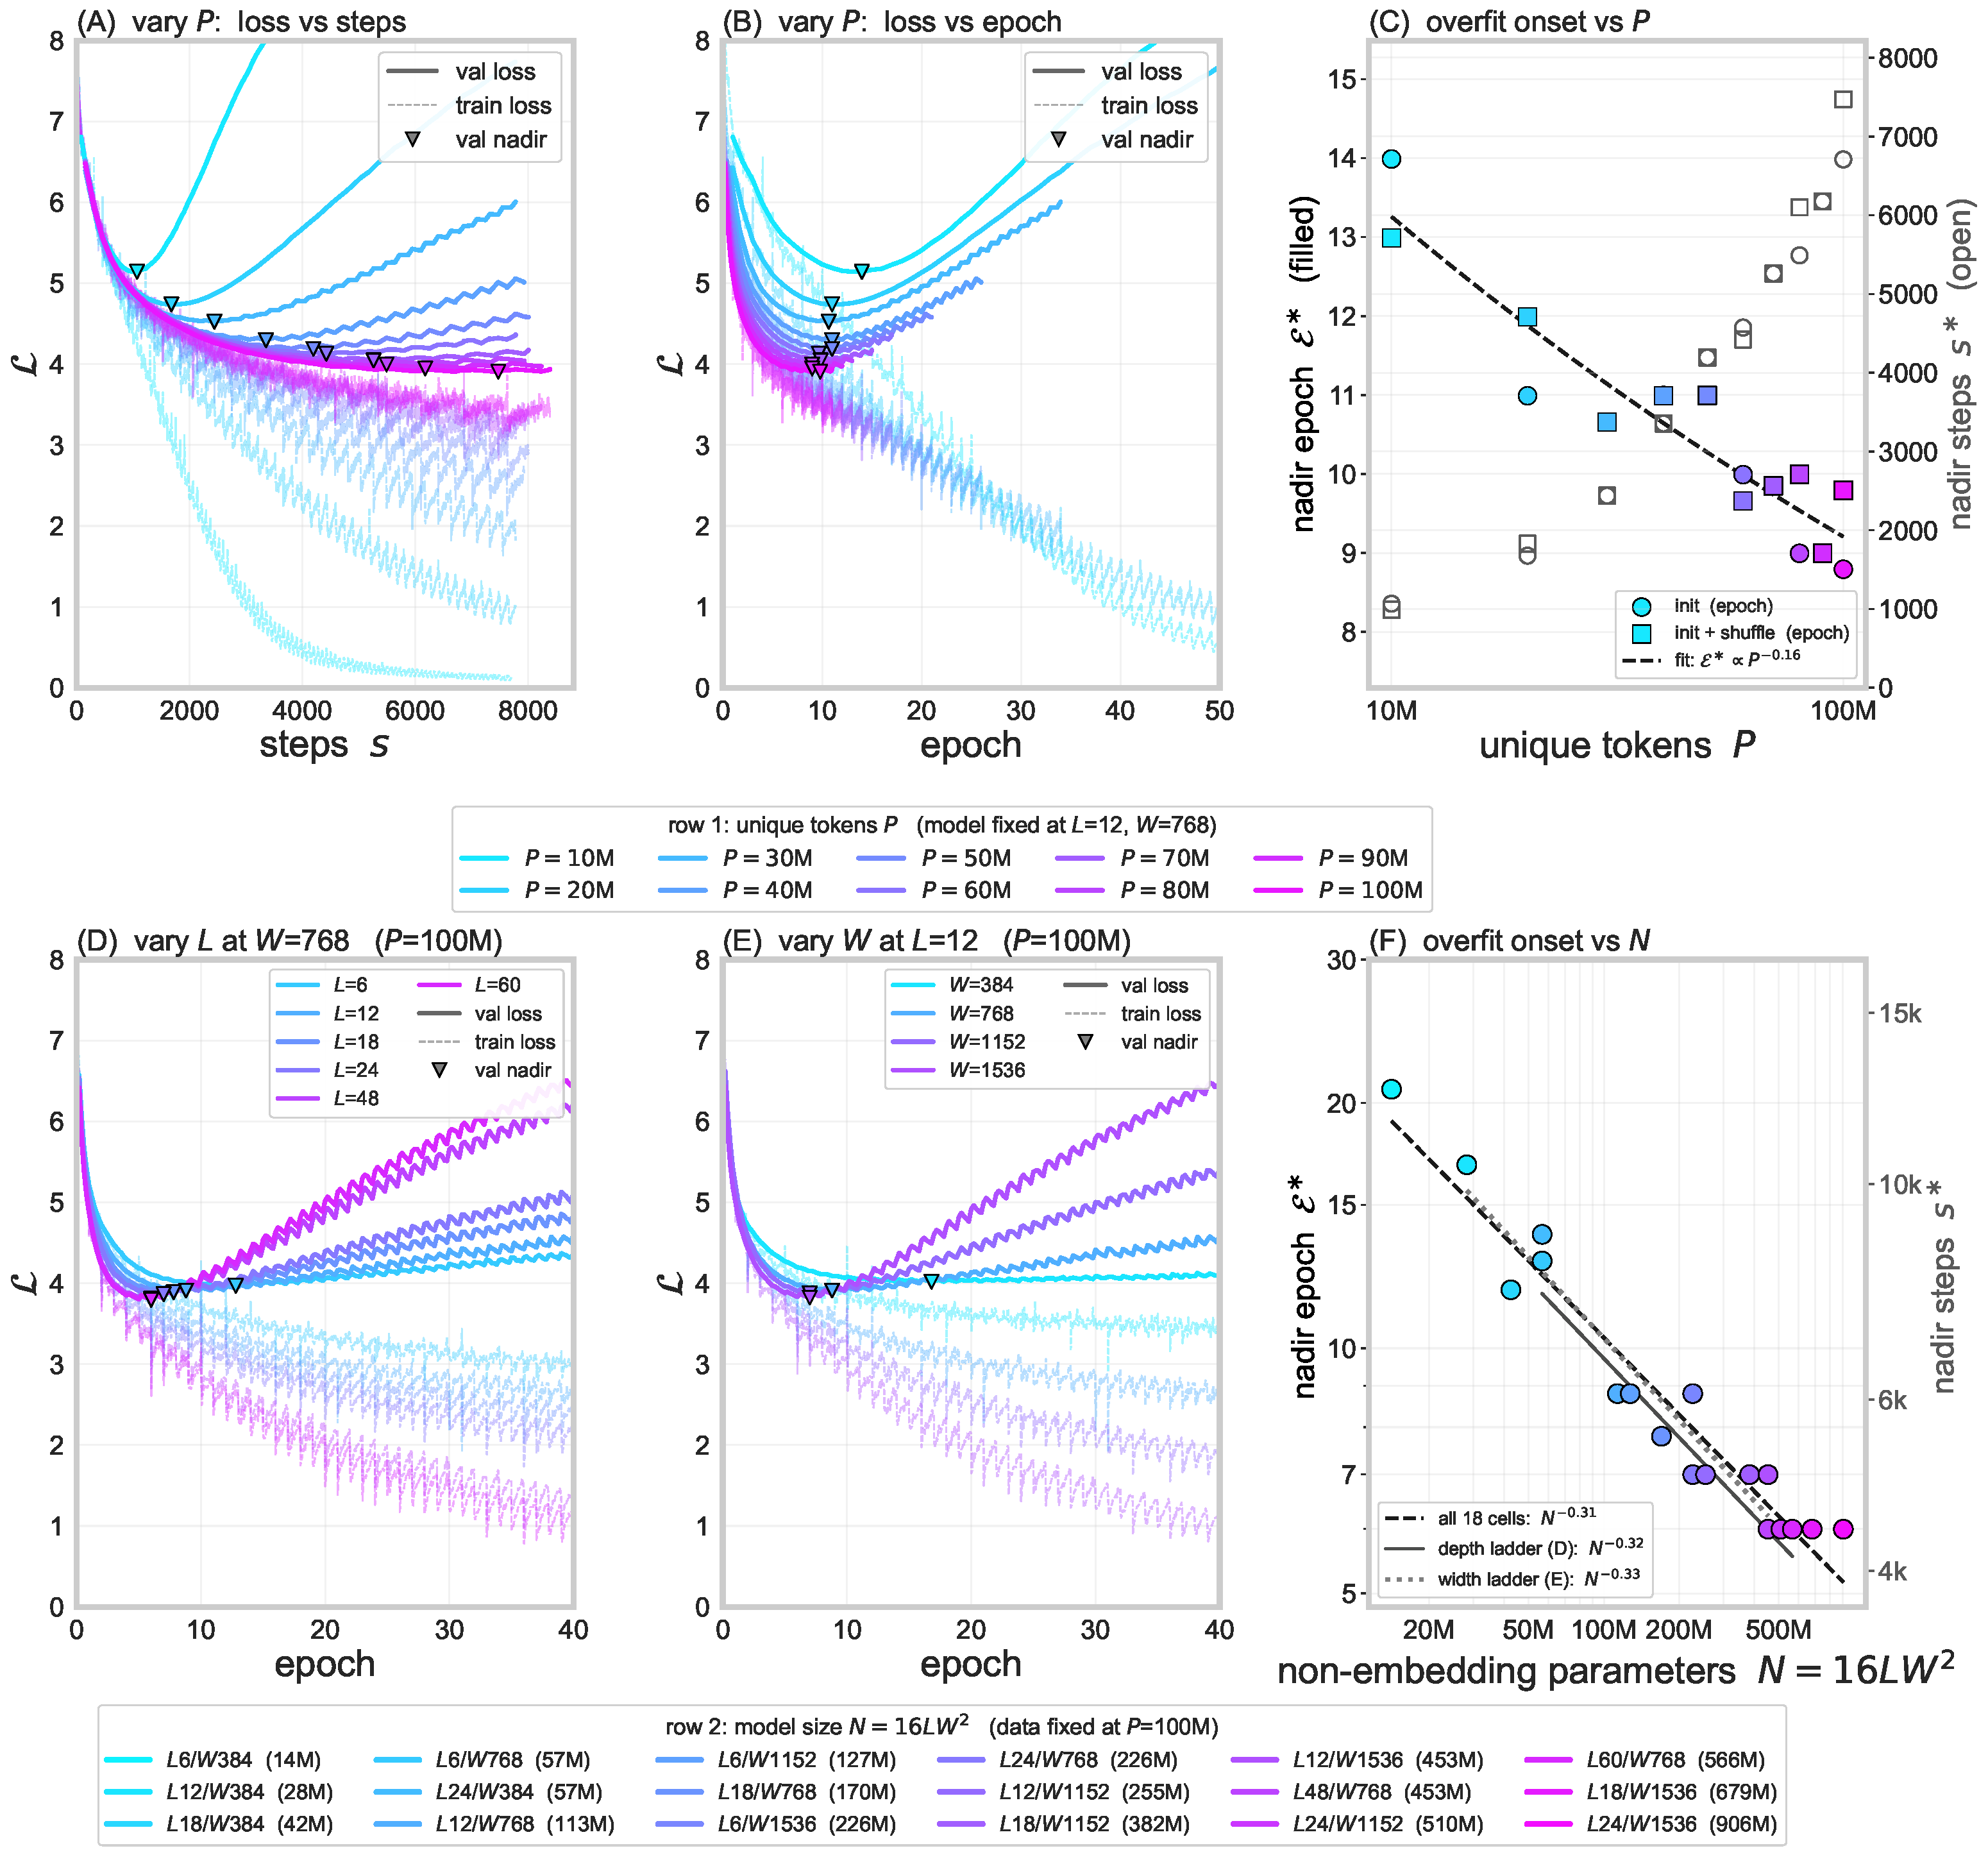
\includegraphics[width=\linewidth]{experiments/figures/10_sister_panels/expt_fig1_sister_panels.pdf}
  \caption{%
    Multi-epoch training produces late-time overfitting along both the data axis
    (top row) and the model-size axis (bottom row).
    \textbf{Top}, fixed model $L{=}12,W{=}768$, varying unique tokens $P$:
    (A) validation loss (solid) and training loss (dashed) versus global step for
    $P\in\{10,\ldots,100\}$M, triangles marking the best validation checkpoints;
    (B) the same curves in epochs; (C) the optimal stopping position versus $P$,
    in epochs (filled, left axis) and steps (open, right axis).
    \textbf{Bottom}, fixed data $P{=}100$M, varying $N=16LW^2$ over a $40\times$
    range: (D) depth ladder at $W{=}768$; (E) width ladder at $L{=}12$;
    (F) optimal stopping epoch (filled) and attained minimum $\mathcal L^*$
    (open) versus $N$. The optimal epoch count is only weakly sensitive to $P$
    ($\mathcal E^*\propto P^{-0.16}$) but falls steeply in model size
    ($\mathcal E^*\propto N^{-0.43}$; $N^{-0.33}$ on the $L{=}12$ row alone).
    All runs use $\lambda{=}0$ and a constant learning rate.
  }
  \label{fig:datasize_sweep}
\end{figure}

\begin{figure}[t]
  \centering
  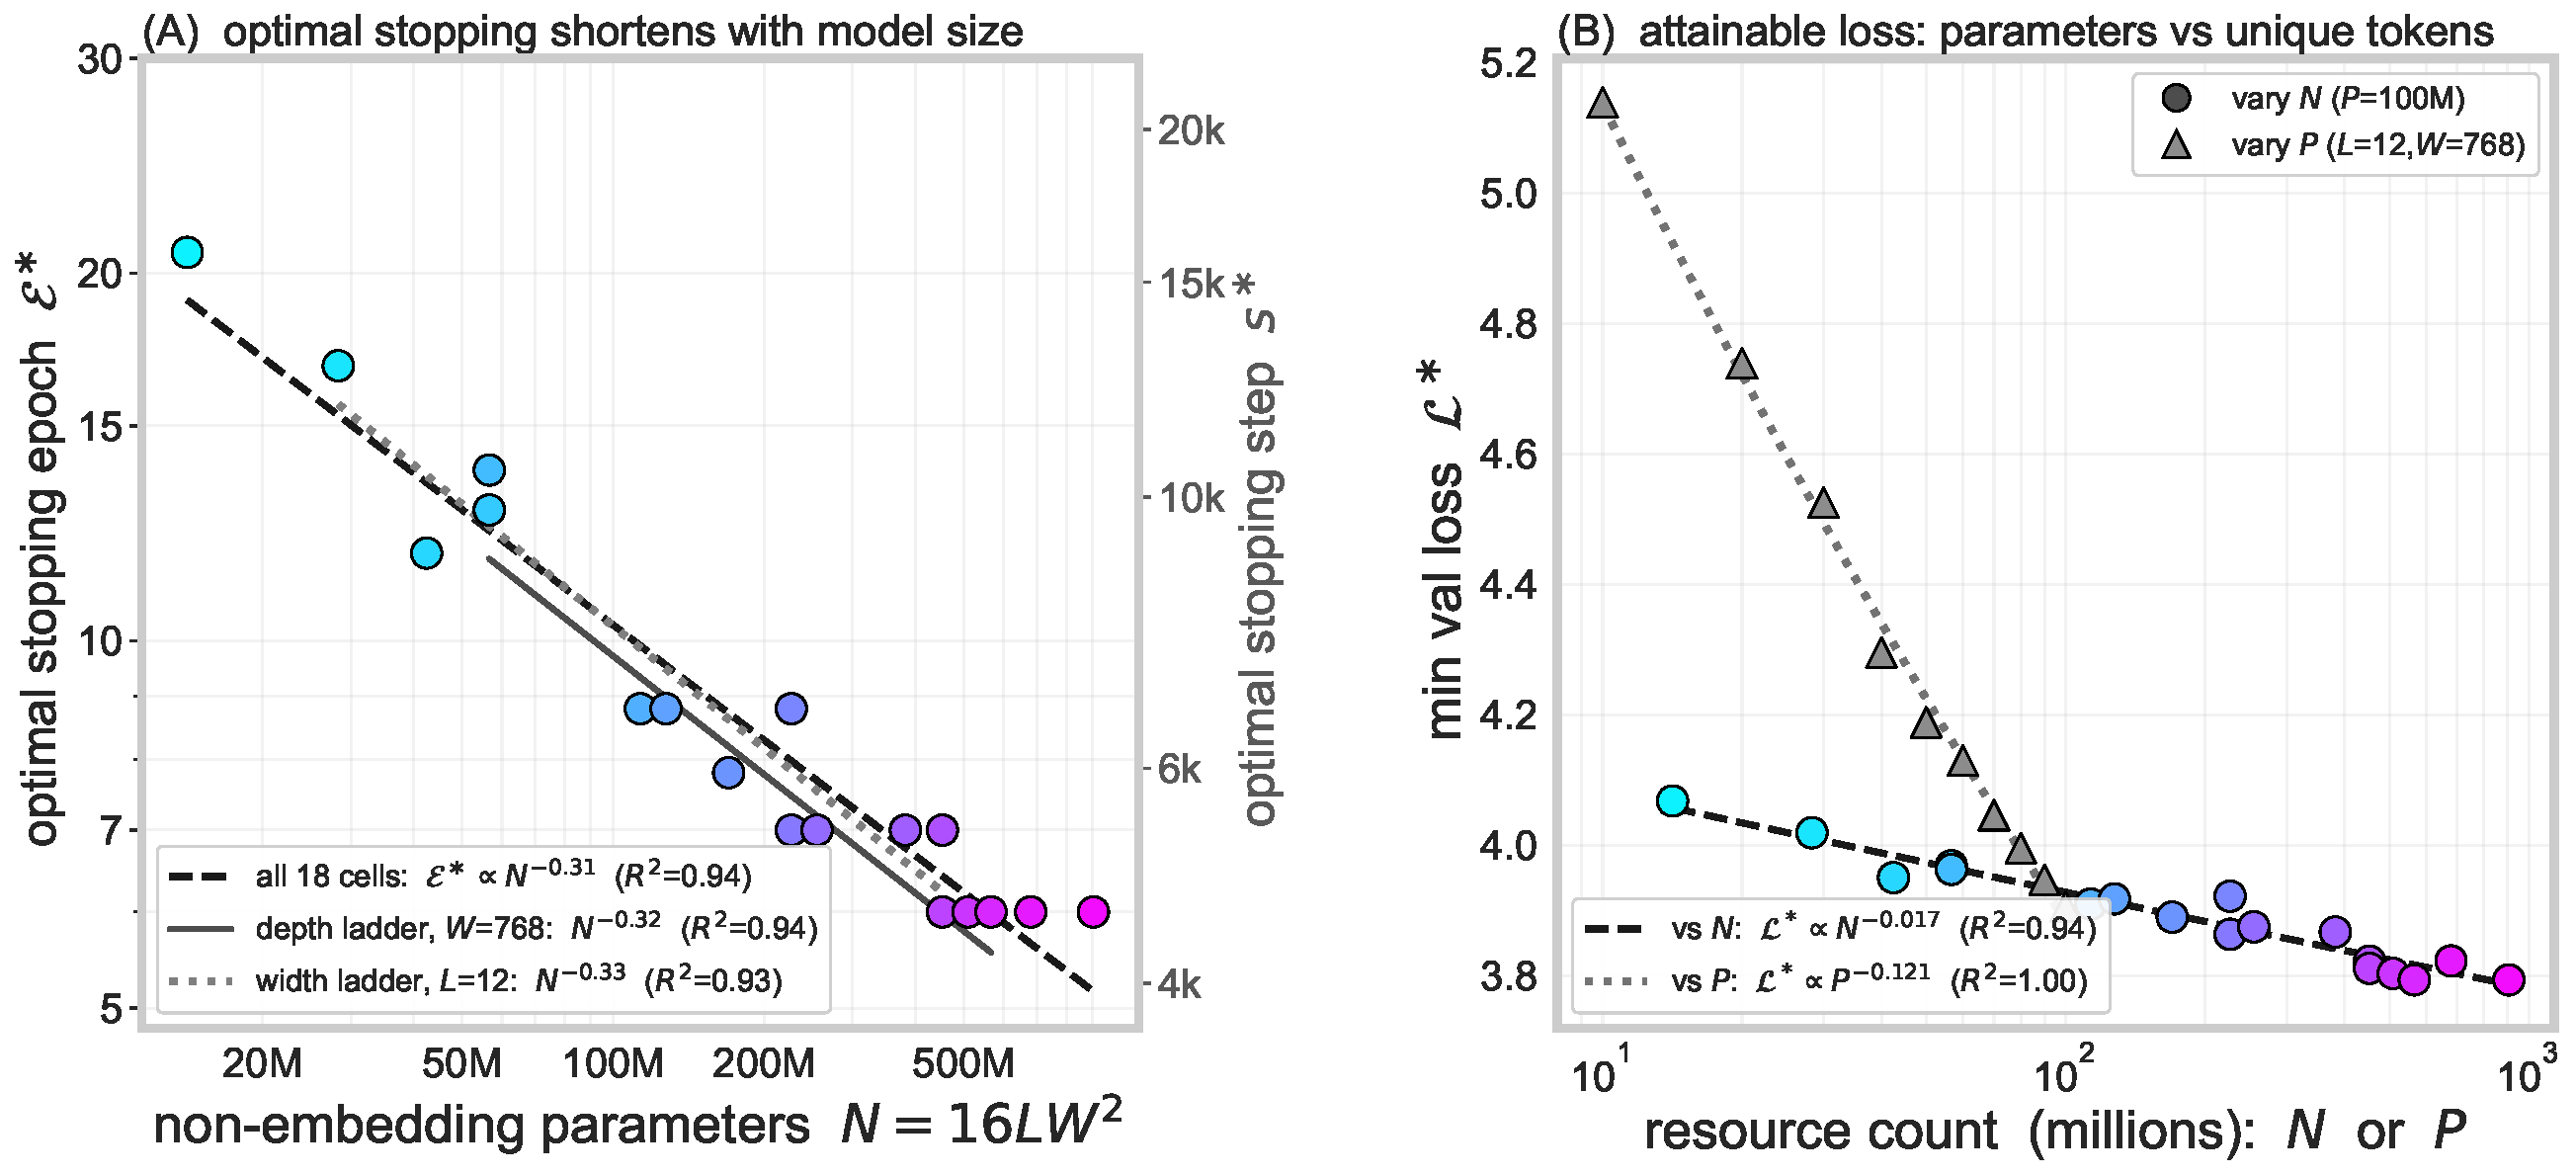
\includegraphics[width=\linewidth]{experiments/figures/10_sister_panels/expt_optimal_stopping.pdf}
  \caption{%
    Optimal stopping and attainable loss versus model size, from the 12 cells at
    $P{=}100$M. (A) The optimal stopping epoch $\mathcal E^*$ follows a power law
    in $N=16LW^2$; the right axis relabels the same quantity in optimizer steps
    (763 steps per epoch at $P{=}100$M). The dashed fit uses all 12 cells, the
    dotted fit only the $L{=}12$ row. (B) Minimum validation loss against
    parameters (circles) and against unique tokens (triangles), each fit drawn
    over its own measured range.
  }
  \label{fig:optimal_stopping}
\end{figure}


% --- Notes (do not belong in the short captions) ---
%
% Data provenance.
%   Top row: data_export/expt4_datasize/wd0_fixed_tokens/ (10 df x 2 strategies,
%   lambda=0, constant LR, ~1B-token budget each). The two ensembling strategies
%   are averaged per df for panels A and B and shown separately in panel C.
%   Bottom row: experiments/logs/fd_{train,gridfill,widthext}_d*_w*_*_0.out,
%   model 0 only, df=1.0, lambda=0, constant LR, E=1. Same 12 cells as
%   expt_fig5_model_size_law.py, so the two figures share every L* value.
%
% Why panels D/E use the epoch axis only.
%   At fixed P the step axis is the epoch axis rescaled by 763 steps/epoch, so a
%   second axis would carry no information. This is not true of row 1, where P
%   varies and the epoch axis is what collapses the curves.
%
% Provisional depth exponent.
%   The depth axis of the bottom row was measured before the CompleteP
%   residual-path correction (unlimited/train.py, commit c660582): the depth
%   factor L_base/L reached the attention and MLP branches but not the
%   x0-injection or U-Net skip paths. The correction is exactly the identity at
%   L = L_base = 12, so the L=12 row is unaffected; that is why alpha = 0.332 is
%   quoted alongside the full-grid alpha = 0.426, and why the depth runs should
%   be repeated before the full-grid exponent is treated as final.
%
% Comparability of the two attainable-loss exponents.
%   alpha_N = 0.187 and alpha_P = 0.178 look nearly equal, but the fitted
%   asymptotes differ sharply (L_inf = 3.539 vs 1.414). They describe approach
%   rates to different floors and must not be read as an equivalence between a
%   parameter and a token.
